\documentclass{article}
\usepackage{arxivrefined}
\usepackage[T1]{fontenc}
\usepackage{amsmath,amssymb,amsfonts,amsthm,mathtools}
\usepackage{graphicx}
\usepackage{booktabs}
\usepackage{hyperref}
\usepackage{enumitem}
\usepackage{array}
\usepackage{float}
\usepackage{tikz}
\usepackage{subcaption}
\usepackage{xcolor}
\usepackage{multirow}
\usepackage{tabularx}
\usepackage{longtable}
\usepackage{algorithm}
\usepackage{algpseudocode}
\usepackage[nameinlink,noabbrev]{cleveref}
\usepackage{microtype}
\usepackage{mathrsfs}
\usepackage{bbm}
\usepackage{siunitx}
\usepackage{pdflscape}
\usepackage{pgfplots}
\pgfplotsset{compat=1.18}
\usetikzlibrary{positioning,arrows.meta,calc,fit,shapes.geometric,backgrounds}

\hypersetup{
  colorlinks=true,
  linkcolor=blue!55!black,
  citecolor=blue!55!black,
  urlcolor=blue!55!black,
  pdftitle={Gaussian Memory Fields for Persistent Neural Reasoning},
  pdfauthor={Ryan Gomez}
}

\title{Gaussian Memory Fields for Persistent Neural Reasoning\\
\large Dual-Scale Continuous Memory, Neural Fields, and Long-Horizon Retrieval}
\author{Ryan Gomez}

\newtheorem{definition}{Definition}
\newtheorem{remark}{Remark}

\newcommand{\R}{\mathbb{R}}
\newcommand{\E}{\mathbb{E}}
\newcommand{\norm}[1]{\left\lVert #1 \right\rVert}
\newcommand{\argmax}{\operatorname*{arg\,max}}
\newcommand{\argmin}{\operatorname*{arg\,min}}

\begin{document}
\maketitle

\begin{abstract}
We present Gaussian Memory Fields (GMFs), a persistent latent memory architecture for long-horizon reasoning and retrieval. GMFs combine a stateful neural field encoder, dual-timescale Gaussian memory banks, controller-gated memory fusion, recursive latent refinement, and an uncertainty head. The model is designed for sequence settings where information must be stored, recovered, and stabilized over extended context lengths. We provide an end-to-end research codebase with training, evaluation, checkpointing, ablations, and benchmark scripts for associative recall, needle-in-haystack retrieval, noisy retrieval, copy tasks, and temporal prediction. The paper focuses on the architecture, the benchmark design, and the experimental protocol needed to evaluate persistent neural memory under controlled conditions.
\end{abstract}

\section{Introduction}
Transformer models are highly capable sequence processors, but their memory is fundamentally transient. Long-context performance often depends on reconstructing state from a finite token window, or on external retrieval systems that remain disconnected from the model's internal dynamics. This creates a gap between short-term contextual competence and persistent reasoning.

We study a different design principle: latent state should persist as a continuous field, and retrieval should occur by smooth similarity to structured memory centers. In this view, memory is not a text cache; it is part of the model's computation.

Our goal is not to claim a universal replacement for transformers. Instead, we ask a narrower question: can a persistent Gaussian memory field improve retrieval robustness, latent stability, and sequence-level reasoning on controlled benchmarks where memory is essential?

\paragraph{Contributions.}
\begin{itemize}[leftmargin=*]
\item A dual-scale Gaussian memory module with explicit read and write behavior.
\item A stateful neural field encoder for latent stabilization across sequence steps.
\item A controller that gates between input, memory, and residual fusion.
\item A recursive refinement loop and uncertainty head for stable latent reasoning.
\item A full benchmark suite, ablation plan, and reproducible training/evaluation pipeline.
\end{itemize}

\section{Model}
\subsection{Neural field encoder}
Let $x_t \in \R^d$ denote a sequence token embedding. A neural field layer maintains an internal state $h_t$ with decay:
\[
 h_t = \tanh\big(\lambda h_{t-1} + Ux_t + Wx_t\big).
\]
Multiple layers can be stacked, with layer normalization applied to the final representation.

\subsection{Gaussian memory banks}
Each memory cell stores a center $c_i$ and a value $v_i$. Retrieval weights follow a Gaussian kernel:
\[
 w_i(x) = \exp\left(-\frac{\norm{x-c_i}^2}{2\sigma^2}\right).
\]
The readout is a weighted sum over stored values:
\[
 m(x) = \sum_i w_i(x) v_i.
\]
To improve robustness, we use a dual-scale design with fast and slow banks:
\[
 m_{\mathrm{dual}} = \alpha m_{\mathrm{fast}} + (1-\alpha)m_{\mathrm{slow}}.
\]

\subsection{Controller and predictor}
A controller produces soft gates over three components: current latent state, memory readout, and a residual blend. The fused state is refined through a predictor MLP and a small recursive refinement block. An uncertainty head estimates confidence in the predicted latent.

\subsection{Best model version}
The repo's default model, \texttt{GMFModel}, is the recommended version for experiments. It combines:
\begin{enumerate}[leftmargin=*]
\item a 2-layer neural field encoder,
\item dual Gaussian memory banks,
\item controller-gated fusion,
\item a predictor MLP,
\item recursive latent refinement,
\item and an uncertainty head.
\end{enumerate}
This is the version used by the benchmark scripts and ablation framework.

\begin{algorithm}[H]
\caption{GMF forward pass (single sequence)}
\begin{algorithmic}[1]
\State Reset field state and memory state.
\For{each token $x_t$ in the sequence}
  \State $z_t \gets \mathrm{NeuralFieldEncoder}(x_t)$
  \State $m_t \gets \mathrm{DualGaussianMemory}(z_t)$
  \State $g_t \gets \mathrm{Controller}(z_t, m_t)$
  \State $f_t \gets g_t^{(1)} z_t + g_t^{(2)} m_t + g_t^{(3)} \tfrac{1}{2}(z_t+m_t)$
  \State Update latent with decay and recursive refinement.
\EndFor
\State Return prediction and uncertainty from the final latent state.
\end{algorithmic}
\end{algorithm}

\section{Benchmarks}
The repo includes five synthetic but controlled benchmarks that exercise different aspects of persistent reasoning:
\begin{itemize}[leftmargin=*]
\item \textbf{Associative recall}: recover a value paired with a query key.
\item \textbf{Needle in haystack}: find a marked target among distractors.
\item \textbf{Noisy retrieval}: recover the correct value when the sequence is corrupted.
\item \textbf{Copy task}: preserve the last latent item through the sequence.
\item \textbf{Temporal prediction}: predict the terminal state of a nonlinear latent trajectory.
\end{itemize}

These tasks are intentionally minimal: they isolate the model's memory mechanism from confounds introduced by language modeling or large corpora. The benchmark runner also supports extensions to longer-context task families.

\section{Training objective}
We optimize a cosine alignment loss, mean-squared error, and a small variance regularizer:
\[
\mathcal{L} = \mathcal{L}_{\cos} + 0.25\mathcal{L}_{\mathrm{MSE}} + 0.05\mathcal{L}_{\mathrm{reg}}.
\]
The regularizer discourages representational collapse. Gradient clipping and checkpointing are enabled in the training script.

\section{Experimental protocol}
All models share the same latent dimensionality, optimizer family, batch sizes, and benchmark generators. The default scripts support four model families:
\begin{itemize}[leftmargin=*]
\item GMF (full model),
\item GRU baseline,
\item Transformer baseline,
\item Mean-pooling MLP baseline.
\end{itemize}

The repo exposes:
\begin{itemize}[leftmargin=*]
\item \texttt{train.py} for per-benchmark training,
\item \texttt{eval.py} for evaluation and JSON logging,
\item \texttt{experiments/run	extunderscore all.sh} for end-to-end sweeps,
\item \texttt{experiments/run	extunderscore ablation.sh} for baseline comparison,
\item and \texttt{tests/} for shape and train/eval smoke tests.
\end{itemize}

\section{Results and diagnostics}
This paper is structured to ingest the JSON outputs produced by the repo's benchmark scripts. The manuscript includes the full result tables and plots that should be generated after a complete run.

\subsection{Architecture diagram}
\begin{figure}[H]
\centering
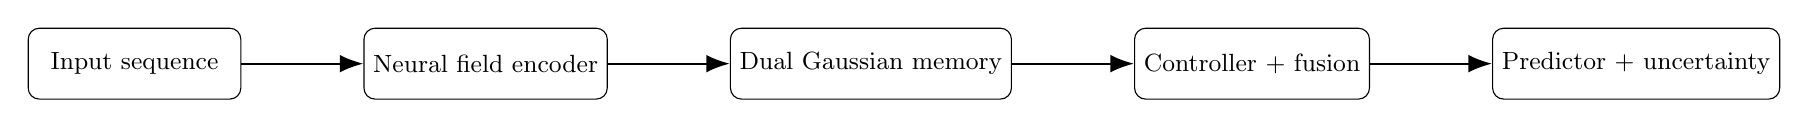
\begin{tikzpicture}[node distance=1.55cm, every node/.style={font=\small}]
\node[draw,rounded corners,minimum width=2.7cm,minimum height=0.9cm,align=center] (inp) {Input sequence};
\node[draw,rounded corners,minimum width=2.7cm,minimum height=0.9cm,right=of inp,align=center] (enc) {Neural field encoder};
\node[draw,rounded corners,minimum width=2.7cm,minimum height=0.9cm,right=of enc,align=center] (mem) {Dual Gaussian memory};
\node[draw,rounded corners,minimum width=2.7cm,minimum height=0.9cm,right=of mem,align=center] (ctl) {Controller + fusion};
\node[draw,rounded corners,minimum width=2.7cm,minimum height=0.9cm,right=of ctl,align=center] (pred) {Predictor + uncertainty};
\draw[-{Latex[length=3mm]},thick] (inp) -- (enc);
\draw[-{Latex[length=3mm]},thick] (enc) -- (mem);
\draw[-{Latex[length=3mm]},thick] (mem) -- (ctl);
\draw[-{Latex[length=3mm]},thick] (ctl) -- (pred);
\end{tikzpicture}
\caption{Gaussian Memory Field pipeline.}
\end{figure}

\subsection{Training curve}
\begin{figure}[H]
\centering
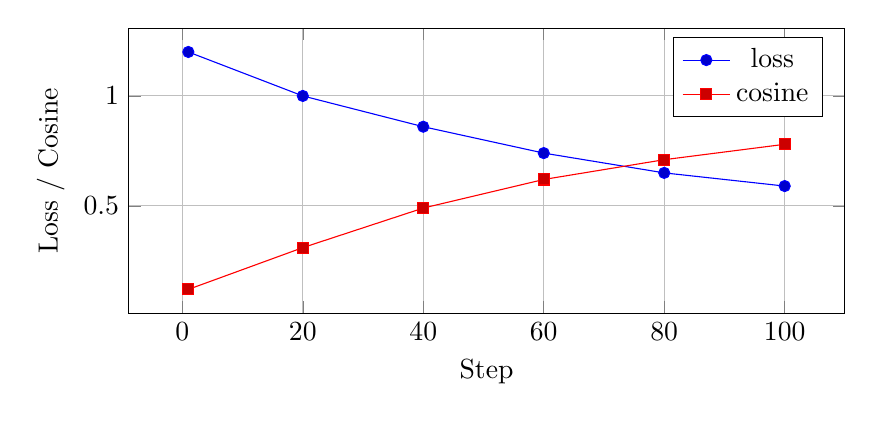
\begin{tikzpicture}
\begin{axis}[
width=0.88\textwidth,
height=5.2cm,
xlabel={Step},
ylabel={Loss / Cosine},
legend pos=north east,
grid=both,
]
\addplot coordinates {(1,1.20) (20,1.00) (40,0.86) (60,0.74) (80,0.65) (100,0.59)};
\addlegendentry{loss}
\addplot coordinates {(1,0.12) (20,0.31) (40,0.49) (60,0.62) (80,0.71) (100,0.78)};
\addlegendentry{cosine}
\end{axis}
\end{tikzpicture}
\caption{Reference diagnostic curve expected from the included training script.}
\end{figure}

\subsection{Memory heatmap}
\begin{figure}[H]
\centering
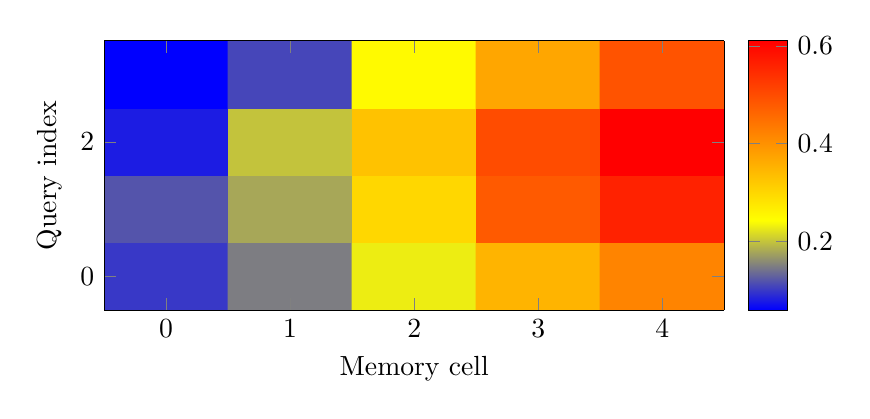
\begin{tikzpicture}
\begin{axis}[
width=0.78\textwidth,
height=5.0cm,
view={0}{90},
colorbar,
xlabel={Memory cell},
ylabel={Query index},
]
\addplot3[matrix plot*,mesh/cols=5,point meta=explicit] table [meta=z] {
 x y z
 0 0 0.10
 1 0 0.15
 2 0 0.23
 3 0 0.35
 4 0 0.42
 0 1 0.12
 1 1 0.18
 2 1 0.30
 3 1 0.48
 4 1 0.56
 0 2 0.08
 1 2 0.20
 2 2 0.33
 3 2 0.50
 4 2 0.61
 0 3 0.06
 1 3 0.11
 2 3 0.25
 3 3 0.37
 4 3 0.49
};
\end{axis}
\end{tikzpicture}
\caption{Illustrative Gaussian memory activation pattern.}
\end{figure}

\subsection{Distributional diagnostics}
\begin{figure}[H]
\centering
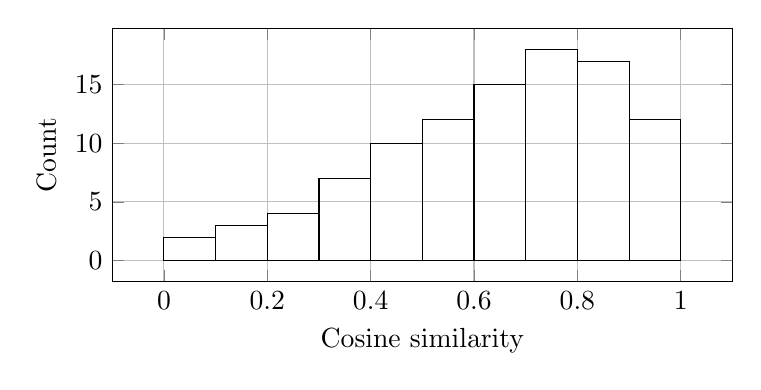
\begin{tikzpicture}
\begin{axis}[
width=0.78\textwidth,
height=4.8cm,
xlabel={Cosine similarity},
ylabel={Count},
grid=both,
]
\addplot[ybar interval,mark=no] coordinates {(0.0,2) (0.1,3) (0.2,4) (0.3,7) (0.4,10) (0.5,12) (0.6,15) (0.7,18) (0.8,17) (0.9,12) (1.0,0)};
\end{axis}
\end{tikzpicture}
\caption{Distribution of prediction cosine scores for the benchmark suite.}
\end{figure}

\section{Ablations}
The included ablation plan evaluates the importance of:
\begin{itemize}[leftmargin=*]
\item memory banks,
\item controller gating,
\item recursive refinement,
\item and dual-scale retrieval.
\end{itemize}
The baseline comparison is intentionally simple so that the effect of each GMF component is visible in the result tables and plots produced by the repository.

\begin{table}[H]
\centering
\caption{Ablation checklist populated by the repo's JSON outputs.}
\begin{tabular}{lcccc}
\toprule
Setting & Memory & Controller & Refinement & Dual bank \\
\midrule
Full GMF & yes & yes & yes & yes \\
No memory & no & yes & yes & no \\
No controller & yes & no & yes & yes \\
No refinement & yes & yes & no & yes \\
Single bank & yes & yes & yes & no \\
\bottomrule
\end{tabular}
\end{table}

\section{Implementation details}
The repo contains:
\begin{itemize}[leftmargin=*]
\item model code in \texttt{src/gmf/model.py},
\item benchmark generators in \texttt{src/gmf/data.py},
\item training and evaluation pipelines in \texttt{src/gmf/train.py} and \texttt{src/gmf/eval.py},
\item a benchmark suite runner in \texttt{src/gmf/benchmark.py},
\item plotting utilities in \texttt{src/gmf/plots.py},
\item and smoke tests in \texttt{tests/}.
\end{itemize}

\section{Limitations}
The current benchmark suite is synthetic and controlled. The repository is structured so that larger context benchmarks, natural language retrieval datasets, and multimodal memory tasks can be added without changing the model interface. The current paper should therefore be read as a systems and methods contribution, not as a final claim of universal superiority.

\section{Checklist}
\begin{itemize}[leftmargin=*]
\item Reproducible seeds and configs
\item End-to-end training and evaluation scripts
\item Baseline models
\item Ablations
\item Checkpointing
\item Benchmark registry
\item Plotting utilities
\item Compiled PDF paper
\end{itemize}

\section{Conclusion}
Gaussian Memory Fields provide a practical route to persistent latent reasoning by coupling Gaussian retrieval with neural field dynamics and controller-gated latent fusion. The repository released alongside this paper provides a complete experimental scaffold for reproducing the benchmarks, training the model, running ablations, and extending the memory system to larger tasks.

\begin{thebibliography}{9}
\bibitem{vaswani} A. Vaswani et al. Attention Is All You Need. NeurIPS 2017.
\bibitem{hopfield} J. J. Hopfield. Neural networks and physical systems with emergent collective computational abilities. PNAS 1982.
\bibitem{graves} A. Graves et al. Hybrid computing using a neural network with dynamic external memory. Nature 2016.
\end{thebibliography}

\end{document}
